\documentclass[10pt]{article}
\usepackage[margin=2cm]{geometry}
\usepackage{amsmath,amssymb}
\usepackage{booktabs}
\usepackage{graphicx}
\usepackage{float}
\usepackage{array,tabularx}
\usepackage[font=small,labelfont=bf]{caption}
\usepackage[compact]{titlesec}
\usepackage{enumitem}
\usepackage{microtype}
\usepackage[hidelinks]{hyperref}
\setlist{itemsep=1pt,topsep=3pt}
\setlength{\parskip}{4pt}
\setlength{\parindent}{0pt}
\graphicspath{{figures/}}
\newcommand{\fig}[1]{Figure~\ref{#1}}
\newcommand{\tab}[1]{Table~\ref{#1}}

\begin{document}
\sloppy

\begin{center}
{\LARGE SuperMimic on Kangaroo, M4 on the cluster: the paper's settings}\\[4pt]
SuperMimic and PPO-Sim for 24\,h each on one Leonardo A100, against the 12\,h local runs of M4.
Branch \texttt{omm/supermimic} of pal\_mjlab, 25 October 2026.
\end{center}

\section*{Summary}

M4's local SuperMimic run oscillated, and its two settings forced by the 16\,GB GPU were the first
suspects. Here SuperMimic ran with the paper's exact settings (TF32, replay 1000) for 24\,h on one A100,
next to PPO-Sim on the same hardware and clock. All four runs share M4's benchmark: every
\texttt{dev} clip (1296) once from its first frame.

\begin{itemize}
  \item \textbf{SuperMimic beats PPO-Sim on equal hardware.}
  \begin{itemize}
    \item It passes PPO-Sim's 24\,h result (15 failures, tracking return 0.770) after \textbf{9.3\,h}.
    \item 25 of its 31 later checkpoints have a higher tracking return.
    \item Its best checkpoint fails \textbf{2} clips with tracking return \textbf{0.872}, and its arm error is
    41\% lower.
    \item It used 15$\times$ less simulator data.
  \end{itemize}
  PPO-Sim runs $2.2\times$ faster on the A100 than locally, but gains only 0.025 in tracking return
  after 6\,h.
  \item \textbf{The oscillation remains.} Over the same iterations the paper's settings give at least as
  many failure spikes as the local run (20 vs 11), with the same critic-first sequence. The benchmark shows collapses of
  101 to 1287 failures at 8.8, 12.2, 14.1 and 21.4\,h. So bf16 and the shorter replay are not
  the cause.
  \item \textbf{A second failure mode late in training.} After iteration 27,000 a few imagined rollouts
  get enormous penalties and the critic's loss explodes (up to $10^{14}$).
  \item \textbf{Speed is our largest gap to the paper:} 0.57 iterations per second on one A100, about
  $8\times$ fewer per GPU than the paper. Our iteration is bound by the BPTT update; about $3\times$ of
  the gap is the H100.
  \item \textbf{One seed per run.} Differences of a few failures are within run-to-run noise.
\end{itemize}

\textbf{Next (Section~\ref{sec:options}).} Speed first: compile the imagination step. Then the
stability candidates, one at a time on the free local GPU; a G1 control; the critic ablation. Only then
spend A100 hours on \texttt{full} and the paper's results. Nothing has been changed yet.

\section{The runs}

\textbf{What ran.} Two jobs on CINECA Leonardo, each on one A100 (64\,GB) for 24\,h. Both started at
the same moment from the same code (commit \texttt{9d58dab}) and read the same \texttt{dev} library
(1296 clips, 2.5\,h) from the copy of the dataset on the cluster.
\begin{itemize}
  \item \textbf{SuperMimic} with the paper's settings (Table~A.5): TF32 learning updates and a replay of
  1000 steps per env. These are the two settings the 16\,GB local GPU could not fit (D16): M4's local
  run used bf16 and a replay of 500. Everything else is the same as M4, including the learned failure
  head (D31) and the critic.
  \item \textbf{PPO-Sim}, the model-free baseline: the same environment, trained with BeyondMimic's PPO
  on 8192 envs, unchanged from M1.
\end{itemize}

\textbf{A cluster pitfall, fixed before these runs.} Leonardo's GPU nodes have the 535 driver (CUDA
12.2). Below 12.4, mjlab turns off CUDA graphs and MuJoCo Warp launches its kernels one by one: the
simulator ran about $8\times$ slower (PPO-Sim collection 12.8\,s instead of 1.57\,s per iteration).
Loading the forward-compatibility driver of the \texttt{cuda/12.6} module restores them. The first pair
of jobs ran without it for about an hour; they were cancelled and restarted with the fix.

\begin{table}[H]
\centering\small
\caption{Throughput. Simulator steps: 24 per env per PPO iteration on 8192 envs; about 2.5 per env per
SuperMimic iteration on 4096 envs.}
\label{tab:throughput}
\begin{tabular}{lrrrr}\toprule
run & iterations & hours & iterations/h & sim steps [B] \\\midrule
SuperMimic, cluster & 49,300 & 23.9 & 2,060 & 0.50 \\
SuperMimic, local & 27,510 & 12.0 & 2,296 & 0.28 \\
PPO-Sim, cluster & 38,677 & 24.0 & 1,610 & 7.60 \\
PPO-Sim, local & 8,865 & 12.0 & 739 & 1.74 \\
\bottomrule\end{tabular}

\end{table}

\begin{itemize}
  \item \textbf{The A100 helps PPO-Sim much more than SuperMimic.} PPO-Sim's iterations take 2.2\,s
  instead of 4.9\,s locally (collection 1.54\,s, learning 0.68\,s), so it runs $2.2\times$ more iterations
  per hour. SuperMimic's iteration is 1.78\,s, slightly slower than locally (1.56\,s): the TF32 policy
  update takes 1.37\,s, the world model 0.25\,s and collection 0.16\,s. It is bound by the BPTT update,
  not by the simulator.
  \item \textbf{So the A100 changes the race.} In M4, SuperMimic's advantage was measured against a
  PPO-Sim that ran at 739 iterations per hour. On the A100, PPO-Sim runs 1,610.
  \item \textbf{We are far from the paper's speed.} Under our reading of an iteration (one update, D10),
  the paper's two-GPU run averages about 9 iterations per second, about 4.5 per GPU if it scales
  linearly. Ours does 0.57 on one A100, $8\times$ fewer per GPU. An H100 has about $3\times$ an A100's
  dense TF32 throughput. The remaining $2.5$--$3\times$ is consistent with our imagination loop not being
  compiled (only the kinematics is): an independent reproduction measured $4.5\times$ from compiling
  it.
\end{itemize}

\textbf{How it is compared.} Every SuperMimic checkpoint (every 1000 iterations, about 29\,min) and
every 1000th PPO-Sim iteration (about 37\,min) were benchmarked the paper's way on the local GPU
(\texttt{eval.py}): every \texttt{dev} clip once from its first frame, with no randomization or noise.
That is the protocol of M4, so all four runs share one benchmark. Runs are compared at equal training
hours. Each configuration ran once, so differences of a few failures are within run-to-run noise (M1
measured about 15\% on PPO-Sim's failure count).

\section{Benchmark}

\begin{figure}[H]
\centering
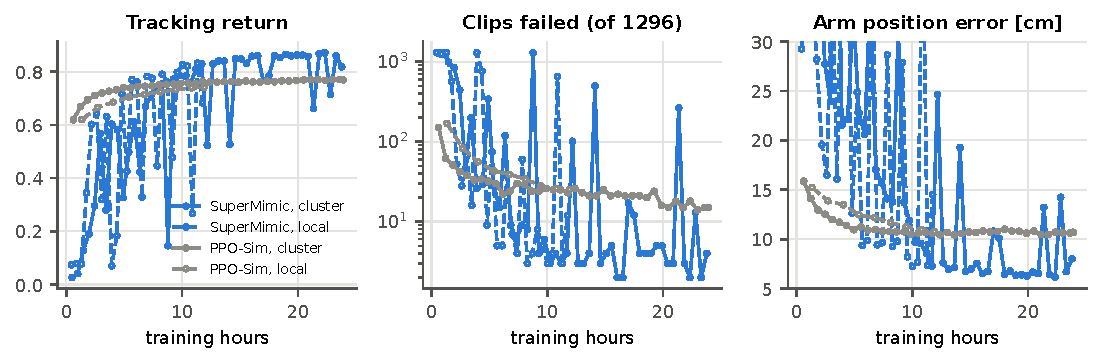
\includegraphics[width=\textwidth]{cluster_benchmark.pdf}
\caption{The paper's benchmark (every \texttt{dev} clip once from its first frame) of each checkpoint vs
training hours. Solid: the cluster runs (A100, 24\,h). Dashed, open markers: M4's local runs (RTX 5060
Ti, 12\,h). The failure axis is logarithmic; zero failures are drawn at 1.}
\label{fig:benchmark}
\end{figure}

\begin{table}[H]
\centering\small
\caption{Best (highest tracking return) and last checkpoint of each run. Errors are root-relative
body-position errors averaged over each clip. Every cluster checkpoint is listed in the appendix.}
\label{tab:summary}
\setlength{\tabcolsep}{4pt}
\resizebox{\textwidth}{!}{\begin{tabular}{lrrrrrrr}\toprule
checkpoint & hours & iteration & failed & tracking return & legs [cm] & arms [cm] & torso [cm] \\\midrule
SuperMimic, cluster, best & 22.3 & 46,000 & 2 & 0.872 & 4.4 & 6.2 & 1.8 \\
SuperMimic, cluster, last & 23.8 & 49,000 & 4 & 0.819 & 5.4 & 8.0 & 2.5 \\
\midrule
SuperMimic, local, best & 11.3 & 26,000 & 3 & 0.832 & 5.0 & 7.3 & 1.7 \\
SuperMimic, local, last & 11.8 & 27,000 & 12 & 0.684 & 7.7 & 14.5 & 2.5 \\
\midrule
PPO-Sim, cluster, best & 21.7 & 35,000 & 15 & 0.771 & 6.1 & 10.5 & 2.6 \\
PPO-Sim, cluster, last & 23.9 & 38,500 & 15 & 0.770 & 6.2 & 10.7 & 2.6 \\
\midrule
PPO-Sim, local, best & 11.9 & 8,800 & 25 & 0.742 & 6.4 & 10.8 & 2.4 \\
PPO-Sim, local, last & 11.9 & 8,800 & 25 & 0.742 & 6.4 & 10.8 & 2.4 \\
\bottomrule\end{tabular}
}
\end{table}

\begin{itemize}
  \item \textbf{PPO-Sim on the A100 plateaus early.} It passes its local 12\,h level (0.742) at 6.2\,h
  (0.745, 22 failures), then gains little: 0.770 with 15 failures at 24\,h. Its
  arm error stays near 10.7\,cm.
  \item \textbf{SuperMimic passes PPO-Sim's 24\,h result after 9.3\,h} on the same GPU and clock
  (iteration 19,000: 4 failures, tracking return 0.773). Of its 31 checkpoints from then on, 25 have a
  higher tracking return than PPO-Sim's final policy and 27 fewer failures.
  \item \textbf{It is clearly better at its best.} The best checkpoint (22.3\,h) fails 2 clips with
  tracking return 0.872, against PPO-Sim's best of 15 and 0.771. Its errors are 28\% lower on legs
  (4.4 vs 6.1\,cm), 41\% on arms (6.2 vs 10.5\,cm) and 31\% on torso (1.8 vs 2.6\,cm). The last
  checkpoint fails 4 clips (0.819).
  \item \textbf{It keeps improving where PPO-Sim stalls.} From about 13\,h on, most of its checkpoints
  sit at 0.83--0.87 with 2--5 failures. At 12\,h it matches the local run's best
  (0.831 vs 0.832).
  \item \textbf{But it starts more slowly, and still collapses.} It first passes 0.742 at 8.3\,h
  (locally 5.7\,h; by iteration 17,000 vs 13,000), after a larger start-up transient (Section~3). Until
  about 8\,h PPO-Sim has the higher tracking return, though SuperMimic has fewer failures from 6.9\,h
  outside collapses.
  Six of the 31 checkpoints after 9.3\,h fall below PPO-Sim's final return: two collapses below 0.6
  (25,000 and 29,000), one at 0.662 with 263 failures (44,000), and three dips.
  \item \textbf{With 15$\times$ less simulator data:} 0.50 billion steps against PPO-Sim's 7.6 billion.
\end{itemize}

\section{Stability}

\begin{figure}[H]
\centering
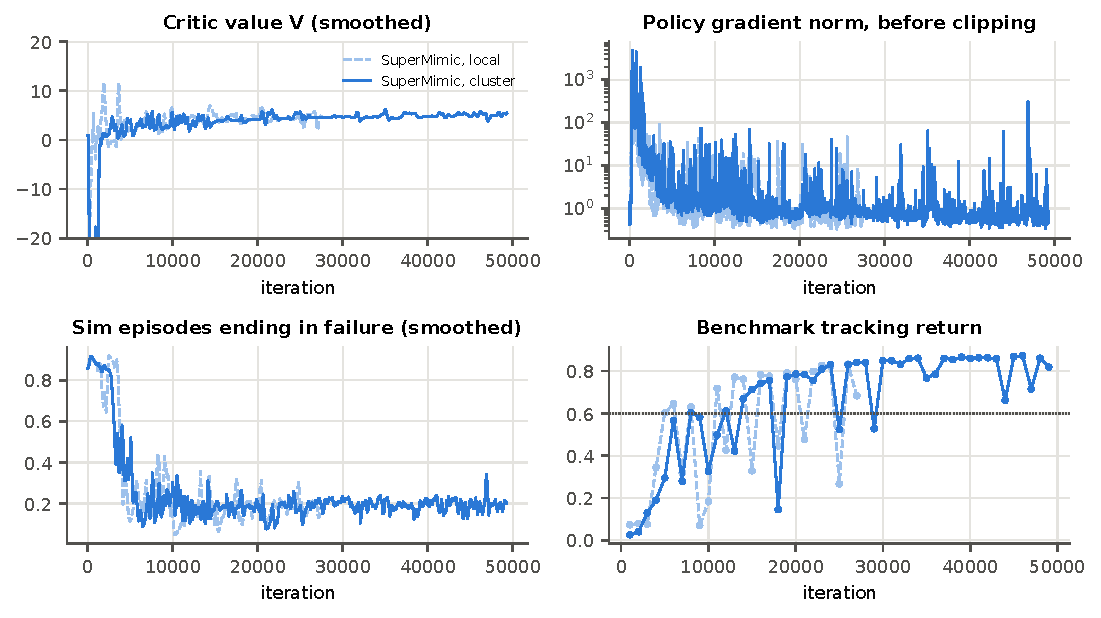
\includegraphics[width=\textwidth]{cluster_stability.pdf}
\caption{SuperMimic on the cluster (solid) and locally (dashed, lighter) by iteration. Top: the critic's
value of the imagined start states (moving average) and the norm of the policy gradient before
clipping. Bottom: share of simulator episodes ending in a failure (moving average), and the benchmark's
tracking return; the dotted line marks 0.6.}
\label{fig:stability}
\end{figure}

\textbf{The paper's settings do not remove the oscillation} (\fig{fig:stability}).
\begin{itemize}
  \item \textbf{Failure spikes are at least as frequent as locally.} After iteration 5000 we count the onsets of
  spikes where more than half of the simulator episodes end in a failure. Over iterations 5000--27,000,
  which both runs cover, the cluster run has 20 and the local run 11.
  \item \textbf{Same sequence as in M4.} In 13 of the cluster run's 24 spikes (local: 7 of 11) the
  critic's value had risen above 1.5$\times$ its recent level in the 100 iterations before. The policy
  gradient peaks in the 20 iterations up to the spike, typically at 10--75 (median 0.8 otherwise).
  \item \textbf{The benchmark shows real collapses, not just noisy training signals.} At iteration
  18,000 (8.8\,h) the policy fails every clip but 9; one checkpoint later it fails 4. Smaller collapses
  follow at 25,000 (101 failures), 29,000 (497) and 44,000 (263), and dips at 35,000--36,000 and 47,000
  (12--17 failures).
  \item \textbf{But the spikes become rarer.} Per stretch of about 11,000 iterations, the cluster run
  has 14, 6, 2 and 2 spike onsets. Of its 33 checkpoints after it first reached PPO-Sim's local level,
  3 are in a collapse (tracking return below 0.6), against 4 of 15 for the local run.
  \item \textbf{A second failure mode late in training.} After iteration 27,000, which the local run
  never reached, the critic's loss explodes in 54 logged iterations (normally about 0.03; up to $10^7$
  around iteration 35,300 and $10^{14}$ around 47,000). Around 47,000 the imagined reward per step, averaged over
  the imagined batch, falls from about $+0.05$ to as low as $-18{,}700$. So a few imagined
  rollouts produce enormous penalties, whose $\lambda$-returns then dominate the critic's loss. Only the
  penalty terms of the reward are unbounded (action rate and joint limits), so a few rollouts' actions or
  predicted joints must leave the data. Our logs don't say which. Both bursts fall within the
  benchmark's dips at 35,000--36,000 and 47,000. The local run shows none of this (critic loss at most 15
  after iteration 3000, imagined reward never below $-0.1$).
  \item \textbf{A larger start-up transient.} In the first 2000 iterations the critic's value fell to
  $-277$ (local: $-53$), its loss reached about $10^8$ and the policy gradient about 4800 before
  clipping. Both runs recovered, the cluster run later.
\end{itemize}

\textbf{The world model and the failure head stay accurate}, as in M4. From iteration 5000 on, the imagined and
simulated 32-step returns from the same states correlate at 0.99--1.0 at most checks, dropping briefly
during collapses (to 0.15 at iteration 7500). The learned failure head ranks fresh failures at a median
AUC of 0.998--1.0.

\section{What this tells us}

\begin{enumerate}
  \item \textbf{M4's result holds on equal hardware, against a faster PPO-Sim.} On \texttt{dev},
  PPO-Sim plateaus at about 0.77 and 15--25 failures. SuperMimic passes it after about 9\,h and reaches
  0.87 with 2 failures, with lower errors on every body group.
  \item \textbf{The oscillation is not caused by bf16 or the shorter replay.} With the paper's settings,
  failure spikes are at least as frequent over the same iterations and follow the same critic-first sequence. The
  cause lies in what we do differently from the paper, or in the robot. Option~2 of Section~5 tests our
  differences one at a time, option~3 the robot.
  \item \textbf{Long training brings a second failure mode:} a few imagined rollouts with enormous
  penalties, which blow up the critic's loss. It needs a diagnosis before a fix (option~2e).
  \item \textbf{Speed is now our largest gap to the paper.} SuperMimic is bound by its BPTT update, so
  the A100 brings it nothing. Compiling the imagination step (option~1) is the cheapest way to make every
  later run cheaper.
  \item \textbf{Checkpoints must still be chosen by the benchmark} (D36). The last checkpoint is good
  here (4 failures), but it comes 1\,h after a dip (47,000) and 2.4\,h after a collapse (44,000).
\end{enumerate}

\textbf{M4 gate.}
\begin{itemize}
  \item ``$\geq$ PPO-Sim on \texttt{dev}'': met on the cluster at equal hours from 9.3\,h, and at the
  best checkpoint by a wide margin. The local runs had already met it at the peaks.
  \item Training stability: not met.
  \item The critic ablation is still open (option~4).
\end{itemize}

\section{Options for M5}
\label{sec:options}

Nothing has been changed yet. These are the options, each with what it would tell us and what it costs.
Costs are in local GPU time (free) or A100 hours on Leonardo; one A100 hour is about 8 local budget
hours, and the project has about 4,560 left (96.8\% used).

\begin{table}[H]
\centering\small
\caption{Options for M5, in the suggested order. ``Local'' runs are 12\,h on the RTX 5060 Ti with bf16
and replay 500; this report shows those two settings are not what makes training oscillate.}
\label{tab:options}
\renewcommand{\arraystretch}{1.15}
\newcolumntype{L}{>{\raggedright\arraybackslash}X}
\begin{tabularx}{\textwidth}{@{}LL>{\raggedright\arraybackslash}p{2.7cm}@{}}\toprule
option & what it tells us & cost \\\midrule
\textbf{1. Speed.} Profile one iteration; compile the whole imagination step and the world-model loss
step, not only the kinematics. &
How much of the $8\times$ per-GPU gap to the paper is ours. Every later option gets cheaper by the same
factor (the reproduction measured $4.5\times$ from compiling). &
Code; about 2\,h of local GPU benchmarks. \\
\textbf{2. Stability, one change at a time.}\newline
(a) a calmer sampler: rate 0.05, unvisited bins easy;\newline
(b) a small failure head on the rule's own features (height and tilt change);\newline
(c) the clean previous action in the observation, noise only when executing (D9);\newline
(d) policy learning rate or loss scale ($-J/H$); critic without privileged inputs (D7); frozen critic
normalization (D34);\newline
(e) first, log which reward term and which rollouts give the extreme imagined rewards (action norms,
joint-limit violations). &
Which part of our setup feeds the critic loop. Judged on the benchmark: share of checkpoints in a
collapse, failure spikes, best and last. (a)--(c) are what the reproduction does differently. &
One local run each (free); 4--7 runs. \\
\textbf{3. G1 control (D18).} Our code on mjlab's G1 with the BONES-SEED G1 clips, a
\texttt{dev}-sized subset; the reproduction's curves as reference. &
Whether the oscillation and the speed are Kangaroo-specific or in our implementation. &
G1 task (robot config, kinematics, library); one local run. \\
\textbf{4. Critic ablation and push test} (paper Fig.~4b, \S4.3). &
What the critic buys us beyond $H = 32$, and robustness. Required for the M4 gate. &
One local run; a push-test script. \\
\textbf{5. Multi-GPU.} Average gradients with an explicit all-reduce, learning rate $\times\sqrt{N}$, as
the reproduction does (91\% efficiency on 4 GPUs). &
Needed for the paper's two-GPU result; halves wall-clock time per run. &
Code; about 2 A100\,h to test. \\
\textbf{6. \texttt{full} dataset} (250.9\,h) on the cluster, SuperMimic and PPO-Sim. &
Scaling with data, against PPO-Sim. Unlikely to cure the oscillation: the paper reports stable training
on LAFAN1's 40 clips too. &
24\,A100\,h per run (about 190 local budget hours each). \\
\textbf{7. The paper's two results.} 3\,h on one H100 (25 failures on 129,514 clips); 9.8\,h on two
H100s (zero failures). &
Whether Kangaroo reaches the paper's level. Their numbers are on G1, so they are a reference, not a
target. &
At today's speed: 10--50 and 60--160 A100\,h. After option 1: a third to a quarter of that. \\
\textbf{8. Data sweep} (1, 10, 40\,h), the original M5 plan. &
Compute to a target return vs dataset size (paper Fig.~3b, c). &
Local runs, or 24\,A100\,h each. \\
\bottomrule
\end{tabularx}
\end{table}

\begin{itemize}
  \item \textbf{Why this order.} Option 1 multiplies the value of everything after it, and our largest
  gap to the paper is speed, not tracking. Options 2--4 run on the free local GPU, since this report
  shows the local settings reproduce the oscillation. The cluster budget (about 570 A100\,h) is then kept
  for options 6--7, after the speed work.
  \item \textbf{The ranges in option 7 are wide} because the paper's ``iteration'' is ambiguous (D10: one
  update, or one environment step as the reproduction reads it) and its single-GPU speed is not
  reported.
  \item \textbf{The reproduction} (CuboiLeo/SuperMimic-Reproduced, G1, compared in the
  \texttt{supermimic-compare} worktree, \texttt{docs/supermimic/compare\_reproduced/report.md}) is a
  reference, not a better implementation. Its benchmark divides each clip's return by the steps survived,
  which is optimistic for failing clips, and it has no PPO baseline or ablations yet. Options 1, 2a--c, 3
  and 5 take from its design.
\end{itemize}

\appendix
\section{All cluster checkpoints}

The local runs' checkpoints are listed in M4's report.

\begin{table}[H]
\centering\small
\caption{The paper's benchmark (1296 \texttt{dev} clips) of SuperMimic's cluster checkpoints.}
\label{tab:all-sm}
\begin{tabular}{lrrrrrrr}\toprule
run & hours & iteration & failed & tracking return & legs [cm] & arms [cm] & torso [cm] \\\midrule
SuperMimic & 0.5 & 1,000 & 1295 & 0.026 & 36.7 & 42.0 & 8.4 \\
SuperMimic & 1.0 & 2,000 & 1295 & 0.041 & 23.4 & 36.9 & 10.3 \\
SuperMimic & 1.5 & 3,000 & 990 & 0.129 & 19.4 & 40.1 & 6.4 \\
SuperMimic & 2.0 & 4,000 & 844 & 0.190 & 19.6 & 38.8 & 9.8 \\
SuperMimic & 2.4 & 5,000 & 441 & 0.295 & 15.3 & 27.7 & 4.7 \\
SuperMimic & 2.9 & 6,000 & 46 & 0.567 & 9.9 & 23.9 & 3.6 \\
SuperMimic & 3.4 & 7,000 & 198 & 0.279 & 16.3 & 56.5 & 7.9 \\
SuperMimic & 3.9 & 8,000 & 26 & 0.604 & 9.4 & 21.6 & 3.7 \\
SuperMimic & 4.4 & 9,000 & 29 & 0.582 & 10.5 & 22.2 & 2.9 \\
SuperMimic & 4.9 & 10,000 & 340 & 0.327 & 15.0 & 32.9 & 9.3 \\
SuperMimic & 5.4 & 11,000 & 28 & 0.499 & 13.9 & 22.8 & 4.3 \\
SuperMimic & 5.9 & 12,000 & 15 & 0.612 & 8.7 & 20.6 & 3.1 \\
SuperMimic & 6.4 & 13,000 & 119 & 0.422 & 11.5 & 34.4 & 4.8 \\
SuperMimic & 6.8 & 14,000 & 9 & 0.669 & 7.9 & 17.0 & 3.2 \\
SuperMimic & 7.3 & 15,000 & 6 & 0.713 & 7.3 & 15.7 & 2.4 \\
SuperMimic & 7.8 & 16,000 & 9 & 0.741 & 6.7 & 14.1 & 2.4 \\
SuperMimic & 8.3 & 17,000 & 8 & 0.755 & 7.2 & 13.8 & 2.9 \\
SuperMimic & 8.8 & 18,000 & 1287 & 0.145 & 13.4 & 30.9 & 5.3 \\
SuperMimic & 9.3 & 19,000 & 4 & 0.773 & 6.3 & 13.7 & 2.3 \\
SuperMimic & 9.8 & 20,000 & 6 & 0.786 & 6.1 & 11.9 & 2.2 \\
SuperMimic & 10.2 & 21,000 & 3 & 0.783 & 5.8 & 9.7 & 2.0 \\
SuperMimic & 10.7 & 22,000 & 4 & 0.756 & 6.5 & 9.6 & 2.8 \\
SuperMimic & 11.2 & 23,000 & 3 & 0.810 & 5.4 & 8.6 & 2.6 \\
SuperMimic & 11.7 & 24,000 & 4 & 0.831 & 5.5 & 7.3 & 2.0 \\
SuperMimic & 12.2 & 25,000 & 101 & 0.524 & 10.5 & 24.6 & 5.4 \\
SuperMimic & 12.7 & 26,000 & 3 & 0.830 & 4.9 & 7.6 & 1.9 \\
SuperMimic & 13.1 & 27,000 & 3 & 0.841 & 4.8 & 7.0 & 1.9 \\
SuperMimic & 13.6 & 28,000 & 4 & 0.840 & 5.0 & 7.1 & 1.8 \\
SuperMimic & 14.1 & 29,000 & 497 & 0.528 & 10.0 & 19.3 & 5.4 \\
SuperMimic & 14.6 & 30,000 & 3 & 0.849 & 4.5 & 6.8 & 1.9 \\
SuperMimic & 15.1 & 31,000 & 4 & 0.849 & 4.5 & 7.0 & 1.7 \\
SuperMimic & 15.6 & 32,000 & 5 & 0.832 & 5.0 & 7.6 & 1.8 \\
SuperMimic & 16.0 & 33,000 & 2 & 0.859 & 4.9 & 6.5 & 1.9 \\
SuperMimic & 16.5 & 34,000 & 2 & 0.861 & 4.4 & 6.7 & 1.8 \\
SuperMimic & 17.0 & 35,000 & 17 & 0.767 & 6.2 & 10.8 & 3.1 \\
SuperMimic & 17.5 & 36,000 & 12 & 0.785 & 5.9 & 10.1 & 2.6 \\
SuperMimic & 18.0 & 37,000 & 4 & 0.860 & 4.6 & 6.5 & 1.8 \\
SuperMimic & 18.5 & 38,000 & 4 & 0.854 & 4.9 & 6.8 & 1.9 \\
SuperMimic & 18.9 & 39,000 & 4 & 0.866 & 4.7 & 6.4 & 2.0 \\
SuperMimic & 19.4 & 40,000 & 5 & 0.860 & 5.3 & 6.4 & 1.8 \\
SuperMimic & 19.9 & 41,000 & 5 & 0.863 & 4.8 & 6.3 & 1.7 \\
SuperMimic & 20.4 & 42,000 & 3 & 0.863 & 4.9 & 6.7 & 1.7 \\
SuperMimic & 20.9 & 43,000 & 3 & 0.858 & 4.2 & 6.5 & 1.8 \\
SuperMimic & 21.4 & 44,000 & 263 & 0.662 & 7.5 & 13.2 & 3.1 \\
SuperMimic & 21.8 & 45,000 & 3 & 0.869 & 4.6 & 6.5 & 1.7 \\
SuperMimic & 22.3 & 46,000 & 2 & 0.872 & 4.4 & 6.2 & 1.8 \\
SuperMimic & 22.8 & 47,000 & 13 & 0.715 & 6.1 & 14.2 & 2.5 \\
SuperMimic & 23.3 & 48,000 & 2 & 0.861 & 4.8 & 6.7 & 1.7 \\
SuperMimic & 23.8 & 49,000 & 4 & 0.819 & 5.4 & 8.0 & 2.5 \\
\bottomrule\end{tabular}

\end{table}

\begin{table}[H]
\centering\small
\caption{The same for PPO-Sim's cluster checkpoints (every 1000 iterations and the last).}
\label{tab:all-ppo}
\begin{tabular}{lrrrrrrr}\toprule
run & hours & iteration & failed & tracking return & legs [cm] & arms [cm] & torso [cm] \\\midrule
PPO-Sim & 0.6 & 1,000 & 151 & 0.620 & 8.7 & 15.9 & 3.8 \\
PPO-Sim & 1.2 & 2,000 & 62 & 0.670 & 7.8 & 14.1 & 3.3 \\
PPO-Sim & 1.8 & 3,000 & 51 & 0.695 & 7.3 & 13.0 & 2.8 \\
PPO-Sim & 2.5 & 4,000 & 42 & 0.711 & 7.0 & 12.5 & 2.7 \\
PPO-Sim & 3.1 & 5,000 & 38 & 0.721 & 6.8 & 12.0 & 2.7 \\
PPO-Sim & 3.7 & 6,000 & 33 & 0.727 & 6.6 & 11.7 & 2.6 \\
PPO-Sim & 4.3 & 7,000 & 34 & 0.733 & 6.6 & 11.4 & 2.5 \\
PPO-Sim & 4.9 & 8,000 & 32 & 0.740 & 6.4 & 11.0 & 2.4 \\
PPO-Sim & 5.6 & 9,000 & 30 & 0.739 & 6.4 & 11.3 & 2.4 \\
PPO-Sim & 6.2 & 10,000 & 22 & 0.745 & 6.4 & 10.9 & 2.4 \\
PPO-Sim & 6.8 & 11,000 & 24 & 0.746 & 6.4 & 11.0 & 2.3 \\
PPO-Sim & 7.4 & 12,000 & 30 & 0.747 & 6.3 & 10.8 & 2.4 \\
PPO-Sim & 8.0 & 13,000 & 29 & 0.751 & 6.4 & 10.8 & 2.5 \\
PPO-Sim & 8.7 & 14,000 & 24 & 0.753 & 6.4 & 10.8 & 2.5 \\
PPO-Sim & 9.3 & 15,000 & 24 & 0.754 & 6.3 & 10.8 & 2.5 \\
PPO-Sim & 9.9 & 16,000 & 26 & 0.757 & 6.3 & 10.5 & 2.4 \\
PPO-Sim & 10.5 & 17,000 & 25 & 0.757 & 6.1 & 10.6 & 2.5 \\
PPO-Sim & 11.1 & 18,000 & 25 & 0.756 & 6.3 & 10.7 & 2.4 \\
PPO-Sim & 11.8 & 19,000 & 23 & 0.762 & 6.3 & 10.6 & 2.6 \\
PPO-Sim & 12.4 & 20,000 & 26 & 0.761 & 6.2 & 10.5 & 2.5 \\
PPO-Sim & 13.0 & 21,000 & 23 & 0.761 & 6.2 & 10.7 & 2.5 \\
PPO-Sim & 13.6 & 22,000 & 21 & 0.763 & 6.2 & 10.5 & 2.4 \\
PPO-Sim & 14.3 & 23,000 & 21 & 0.764 & 6.3 & 10.6 & 2.6 \\
PPO-Sim & 14.9 & 24,000 & 25 & 0.761 & 6.3 & 10.7 & 2.5 \\
PPO-Sim & 15.5 & 25,000 & 21 & 0.765 & 6.2 & 10.7 & 2.5 \\
PPO-Sim & 16.1 & 26,000 & 22 & 0.762 & 6.4 & 10.8 & 2.8 \\
PPO-Sim & 16.7 & 27,000 & 21 & 0.762 & 6.3 & 10.7 & 2.7 \\
PPO-Sim & 17.4 & 28,000 & 21 & 0.765 & 6.3 & 10.8 & 2.8 \\
PPO-Sim & 18.0 & 29,000 & 21 & 0.763 & 6.4 & 11.0 & 2.9 \\
PPO-Sim & 18.6 & 30,000 & 20 & 0.766 & 6.2 & 10.8 & 2.6 \\
PPO-Sim & 19.2 & 31,000 & 24 & 0.765 & 6.2 & 10.8 & 2.7 \\
PPO-Sim & 19.9 & 32,000 & 16 & 0.768 & 6.2 & 10.6 & 2.5 \\
PPO-Sim & 20.5 & 33,000 & 15 & 0.769 & 6.2 & 10.8 & 2.7 \\
PPO-Sim & 21.1 & 34,000 & 18 & 0.771 & 6.2 & 10.5 & 2.6 \\
PPO-Sim & 21.7 & 35,000 & 15 & 0.771 & 6.1 & 10.5 & 2.6 \\
PPO-Sim & 22.4 & 36,000 & 18 & 0.768 & 6.2 & 10.7 & 2.7 \\
PPO-Sim & 23.0 & 37,000 & 14 & 0.771 & 6.2 & 10.7 & 2.6 \\
PPO-Sim & 23.6 & 38,000 & 15 & 0.771 & 6.1 & 10.6 & 2.5 \\
PPO-Sim & 23.9 & 38,500 & 15 & 0.770 & 6.2 & 10.7 & 2.6 \\
\bottomrule\end{tabular}

\end{table}

\section{Reproduction}

\begin{footnotesize}
\begin{verbatim}
# job script on Leonardo (after uv sync on the login node; lazyhpc run folder), one per run
module load cuda/12.6 && export LD_LIBRARY_PATH=$CUDA_HOME/compat:$LD_LIBRARY_PATH
srun .venv/bin/python -m pal_mjlab.scripts.supermimic.train Mjlab-SuperMimic-Flat-Pal-Kangaroo-Grippers-ArmWaist1Hz \
  --env.commands.motion.dataset $FAST/omartin1/kangaroo_bones_seed/dataset --env.commands.motion.subset dev \
  --agent.experiment-name supermimic_wm_1hz --agent.run-name dev-paper --agent.save-interval 1000
srun .venv/bin/python -m pal_mjlab.scripts.supermimic.train Mjlab-SuperMimic-PPO-Flat-Pal-Kangaroo-Grippers-ArmWaist1Hz \
  --env.commands.motion.dataset $FAST/omartin1/kangaroo_bones_seed/dataset --env.commands.motion.subset dev \
  --agent.experiment-name supermimic_ppo_sim_1hz --agent.run-name dev-cluster --agent.save-interval 500
# benchmark (local GPU), figures, this report
python -m pal_mjlab.scripts.supermimic.eval --task <task> --checkpoints <run>/model_*.pt --out-dir <dir>
python docs/supermimic/m4/make_cluster_figures.py && (cd docs/supermimic/m4 && latexmk -pdf cluster_report.tex)
\end{verbatim}
\end{footnotesize}

\end{document}
